\documentclass[sigconf,review]{acmart}

\usepackage{microtype}
\usepackage{mathtools}
\usepackage{algorithm}
\usepackage{algorithmic}
\usepackage{enumitem}
\usepackage{placeins}
\usepackage[capitalize,noabbrev]{cleveref}
\usepackage{float}
% Attempt to make hyperref and algorithmic work together better.
\providecommand{\theHalgorithm}{\arabic{algorithm}}

\setcopyright{rightsretained}
\settopmatter{printacmref=true}
\renewcommand\footnotetextcopyrightpermission[1]{}
\makeatletter
\makeatother

\acmConference[KDD '26]{The 32nd ACM SIGKDD Conference on Knowledge Discovery and Data Mining}{August 9--13, 2026}{Jeju, Republic of Korea}
\acmBooktitle{Proceedings of the 32nd ACM SIGKDD Conference on Knowledge Discovery and Data Mining (KDD '26), August 9--13, 2026, Jeju, Republic of Korea}
\acmYear{2026}
\copyrightyear{2026}

\theoremstyle{plain}
\newtheorem{theorem}{Theorem}[section]
\newtheorem{proposition}[theorem]{Proposition}
\newtheorem{lemma}[theorem]{Lemma}
\newtheorem{corollary}[theorem]{Corollary}
\theoremstyle{definition}
\newtheorem{definition}[theorem]{Definition}
\newtheorem{assumption}[theorem]{Assumption}
\theoremstyle{remark}
\newtheorem{remark}[theorem]{Remark}

\newcommand{\maskclassrepolink}{%
  \url{https://github.com/khazum/MaskClass}}
\newcommand{\ccimputedatasetslink}{%
  \url{https://github.com/khazum/ccImputeDatasets}}

\setlist[enumerate]{nosep}
\emergencystretch=1em
\newenvironment{compitemize}
  {\begin{itemize}[noitemsep, topsep=0pt, parsep=0pt, partopsep=0pt]}
  {\end{itemize}}

\begin{document}
\raggedbottom

\title{MaskClass: A Masked Denoising Autoencoder for Scalable and Accurate Single-Cell RNA-seq Analysis}

\author{Marcin Malec}
\email{mamalec@iu.edu}
\affiliation{%
  \institution{Computer Science Department, Indiana University}
  \city{Bloomington}
  \state{Indiana}
  \country{USA}}

\author{Mehmet Dalkilic}
\affiliation{%
  \institution{Computer Science Department, Indiana University}
  \city{Bloomington}
  \state{Indiana}
  \country{USA}}

\author{Hasan Kurban}
\affiliation{%
  \institution{Computer Science Department, Indiana University}
  \city{Bloomington}
  \state{Indiana}
  \country{USA}}
\affiliation{%
  \institution{College of Science and Engineering, Hamad Bin Khalifa University}
  \city{Doha}
  \country{Qatar}}

\renewcommand{\shortauthors}{Malec et al.}

\begin{abstract}
While DNA contains the blueprint of an organism, RNA is the conductor that orchestrates the expression of this blueprint across diverse cellular components; thus, understanding RNA expression holds the key to understanding complex biological systems. The emergence of numerous single-cell RNA sequencing (scRNA-seq) technologies and protocols over the past decade has enabled the study of RNA expression at single-cell resolution with improved accuracy and scalability, now handling gene expression data from hundreds of thousands to millions of cells. However, scRNA-seq data present analytical challenges, including data sparsity, technical noise, and batch effects, which complicate downstream analyses, such as cell clustering and differential expression analysis. To address these challenges, we introduce MaskClass, a masked denoising autoencoder that significantly improves data quality by selectively hiding parts of gene expression data, learning to reconstruct them while minimizing the impact of noisy dropout values, and using a separate process to recover biological zero-expression measurements. While we focus our primary evaluation on scRNA-seq data, the proposed approach is applicable to other high-dimensional, sparse, and noisy data modalities, including other single-cell omics proteomics, spatial transcriptomics, and related domains characterized by structured missing data and measurement noise. Benchmarking against state-of-the-art denoising methods demonstrates MaskClass's effectiveness in noise reduction on simulated data and significant improvement in cell identity clustering across diverse real-world datasets. MaskClass is available as an open source implementation at \maskclassrepolink.
\end{abstract}

\ccsdesc[500]{Applied computing~Life and medical sciences}
\ccsdesc[500]{Computing methodologies~Machine learning approaches}
\ccsdesc[300]{Information systems~Data mining}

\keywords{single-cell RNA-seq, transcriptomics, masked denoising autoencoder, imputation}

\maketitle

\section{Introduction}
\section{Introduction}
Single-cell RNA sequencing (scRNA-seq) enables large-scale measurement of RNA expression across individual cells, enabling exploration of cellular heterogeneity, reconstruction of developmental trajectories, comparison of disease versus non-disease states, and assessment of therapeutic drug response \citep{Hicks2018MissingData, Luecken2019BestPractices, VanDeSande2023DrugDiscovery}. However, only a small amount of RNA transcripts is captured and sequenced during this process, which, combined with the influence of other technical noises, for example, batch effects, results in a highly sparse gene $\times$ cell count matrix \citep{Brennecke2013TechnicalNoise, Hicks2018MissingData}. The zero values can be either biological zeroes indicating no gene expression or missing values, which are referred to as ''dropouts'' \citep{Li2018scImpute,SarkarStephens2021SeparatingMeasurement,Svensson2020NotZeroInflated,Linderman2022ZeroPreserving}. This is the fundamental challenge that complicates downstream analyses, such as clustering, differential expression, and trajectory inference \citep{Luecken2019BestPractices,Hou2020ImputationBenchmark}.

To date, many approaches have been introduced to denoise scRNA-seq data. MAGIC \citep{vanDijk2018MAGIC}, one of the early approaches, uses graph diffusion to smooth expression across similar cells, which has proven effective at recovering global gene-gene interactions, but at the expense of modifying gene values that are not dropout events, including biological zero values\citep{Li2018scImpute,Linderman2022ZeroPreserving,Hou2020ImputationBenchmark}. Statistical approaches such as SAVER \citep{Huang2018SAVER} and scImpute \citep{Li2018scImpute} perform statistical modeling of the counts directly and share counts across genes and cells; however, their performance is highly dependent on modeling assumptions and varies widely across protocols and data-specific properties \citep{Eraslan2019DCA,Li2022AutoClass,Hou2020ImputationBenchmark}.

More recent approaches include autoencoder-based methods such as the deep count autoencoder (DCA) \citep{Eraslan2019DCA} and AutoClass \citep{Li2022AutoClass}. DCA uses a variational autoencoder with a count likelihood and can learn parameters, including dropout and zero-inflation components \citep{Eraslan2019DCA}. AutoClass couples an autoencoder with an auxiliary classifier to better preserve biologically meaningful structures \citep{Li2022AutoClass}. However, like many reconstruction-based approaches, their default outputs typically provide nonzero expression estimates for most gene--cell pairs and do not explicitly enforce the preservation of true biological zeros, which can lead to over-imputation in settings where zero preservation is important \citep{Linderman2022ZeroPreserving,Hou2020ImputationBenchmark}.

In this study, we present MaskClass, a masked autoencoder that denoises scRNA-seq data while preserving the biological signals. Inspired by the success of Masked Autoencoders (MAE) in computer vision and NLP \citep{He2022MAE,Devlin2019BERT}, MaskClass removes noise by selectively masking a portion of gene expression data and reconstructing it from the unmasked expressions. Compared with other state-of-the-art approaches, our method yields more accurate count reconstruction. MaskClass incorporates dual-objective optimization that leverages predictions of biological zeroes to guide the masking process and loss propagation, ensuring that biological zeros are preserved while technical dropouts are recovered. This study makes the following contributions: (1) we adapt masking strategies to the domain of scRNA-seq data; (2) we introduce a biologically aware regularization strategy that minimizes the reconstruction error for dropout values while protecting genuine biological signals; and (3) we demonstrate against state-of-the-art methods, including MAGIC, SAVER, DCA, and AutoClass, that MaskClass achieves the best clustering performance while recovering count expression with minimal MSE.

\section{Related Works}

\subsection{Statistical and Probabilistic Models}

Early methods for scRNA-seq imputation focused on statistical modelling of gene expression counts to separate technical noise from biological signals. Single-cell Analysis Via Expression Recovery (SAVER) \citep{Huang2018SAVER} suggests that the observed unique molecular identifier (UMI) counts for each gene follow a Poisson–Gamma (negative binomial) mixture, and by estimating prior parameters with regression on the most informative genes, SAVER generates a posterior distribution for the latent true expression, allowing the calculation of point estimates and credible uncertainty intervals (UIs). SAVER has shown good performance in recovering distributional properties, such as Gini coefficients, ensuring consistency with independent RNA FISH validation while avoiding erroneous gene–gene correlations. In contrast, scImpute \citep{Li2018scImpute} fits a mixture model to estimate the probability that a zero or low count  corresponds to noise rather than a biological zero. It only imputes values for dropouts with high probability by sharing gene expression from similar cells, which are identified using a subset of genes unlikely to be affected by dropout, thus preserving biological zeros and avoiding changing unaffected gene expression. However, critics suggest that relying on rigid distributional assumptions may introduce bias if the underlying strategy's noise model does not align with the specific sequencing protocol or cell sample \citep{Jiang2022ZeroInflationReview}.

\subsection{Graph-Based and Diffusion Methods} Graph-based methods assume the manifold structure in single-cell data, and compute values assuming that cells with similar expression should contribute to the imputations. MAGIC (Markov Affinity-based Graph Imputation of Cells) \citep{vanDijk2018MAGIC} constructs a $k$-nearest-neighbor affinity graph in a reduced principal component space. It normalizes this graph into a Markov transition matrix, where $M^T$ diffuses information across cellular groups. The imputed matrix is given by $M^t X$, where $X$ is the raw expression matrix. MAGIC has proven effective in recovering nonlinear gene–gene relationships that are otherwise hidden in sparse raw data. However, the diffusion process modifies all data entries, which include non-zero expression values. This global smoothing can eliminate meaningful biological variability if the diffusion parameter $t$ is not well-tuned \citep{Svensson2020NotZI}. In contrast, our previous work, ccImpute \citep{Malec2022ccImpute}, offers an alternative to manifold diffusion by using a consensus clustering strategy. Inspired by SC3 \citep{Kiselev2017SC3}, it computes a cell–cell consensus similarity matrix and imputes likely dropouts by averaging expression across the most similar cells, while minimizing the introduction of new noise and demonstrating better clustering performance than other state-of-the-art approaches.

\subsection{Deep Learning and Autoencoders} The ability to scale and reconstruct non-linear patterns while reducing noise has made autoencoder architectures popular tools for denosing data. The Deep Count Autoencoder (DCA) \citep{Eraslan2019DCA} adapts the standard autoencoder loss function to specific count noise models. Instead of minimizing the Mean Squared Error (MSE), the DCA utilizes a negative binomial (NB) or zero-inflated negative binomial (ZINB) likelihood loss. This allows the model to learn gene-specific means, dispersions, and dropout probabilities while compressing data through a bottleneck layer. DCA scales well to millions of cells and is effective in recovering cell structures with high dropout rates. This allows the selection between NB and ZINB models, acknowledging that UMI-based droplet data may not always require zero-inflation \citep{Svensson2020NotZI}. In contrast, AutoClass \citep{Li2022AutoClass} extends the autoencoder framework by integrating a classifier branch alongside the reconstruction branch stemming from the bottleneck. Trained on pseudo-labels derived from pre-clustering, this dual-branch architecture encourages the bottleneck layer to maintain biologically relevant cluster structures, while the autoencoder reduces noise. Unlike DCA, AutoClass makes no distribution assumptions and can address a wider range of noise sources, such as amplification bias and batch effects, without relying on specific parametric likelihoods.

\subsection{Self-Supervised and Masked Learning} Masked Autoencoders (MAE) have recently achieved state-of-the-art results in areas such as computer vision and natural language processing (e.g., BERT). These methods operate by intentionally masking a portion of the input data and training the model to predict missing values based on the unmasked values, thereby forcing it to learn high-level semantic representations rather than low-level statistics. In this study, we adapted the masking paradigm to scRNA-seq data. In our approach, MaskClass masks portions of the expressed and non-expressed genes at different rates to force the model to learn the underlying structure of gene expression while minimizing the influence of potentially noisy zero counts, distinguishing it from the standard denoising autoencoders discussed above.

\section{Methods}
\label{sec:methods}
\subsection{Experimental scRNA-seq Datasets}
We benchmarked MaskClass against other approaches using five publicly available scRNA-seq datasets, referenced by the first author of their originating publication: Blakeley~\cite{blakeley2015defining}, Pollen~\cite{pollen2014low}, Darmanis~\cite{darmanis2015survey}, Usoskin~\cite{usoskin2015unbiased}, and Li~\cite{li2017reference}. These datasets cover a variety of biological tissues and technical characteristics, as summarized in Table~\ref{tab:datasets}.

The quality of the ground-truth labels varies across these datasets. Blakeley,
Li, and Pollen provide high-fidelity labels derived from controlled
experimental conditions and distinct cell lines, whereas Usoskin and Darmanis
labels were assigned computationally via clustering followed by expert
annotation. To focus the analysis on distinct cellular populations, cells
annotated as "hybrids" in the Darmanis dataset were excluded from benchmarking.

We selected these datasets because they exhibit substantial sparsity and technical noise, making denoising and imputation challenging. In our experiments, we selected the top $1000$ highly variable genes (HVGs) using \texttt{scran} ~\cite{lun2016step}. Raw counts were library-size normalized by scaling each cell to the counts per million (CPM) and applying a $\log_2(X+1)$ transform, with the final log-normalized counts denoted as $\mathbf{X}_{\log}$. Finally, we retained genes expressed in at least three cells.

\begin{table*}[t]
\caption{Summary of the experimental scRNA-seq datasets used for benchmarking. $N$ denotes the number of samples (cells), $M$ the initial number of features (genes) prior to preprocessing, and $K$ the number of distinct cell clusters reported in the original study. Datasets are available at: \ccimputedatasetslink}
\label{tab:datasets}
\centering
\begin{tabular}{@{} l r r r l l @{}}
\toprule
\textbf{Dataset} & \textbf{N (Cells)} & \textbf{M (Genes)} & \textbf{K} & \textbf{Origin} & \textbf{Reference} \\
\midrule
Blakeley & 30 & 16,862 & 3 & Human blastocyst & \cite{blakeley2015defining} \\
Li & 561 & 55,186 & 7 & Human cell lines & \cite{li2017reference} \\
Pollen & 301 & 23,730 & 11 & Human cell lines & \cite{pollen2014low} \\
Darmanis & 420 & 21,516 & 8 & Human cortex & \cite{darmanis2015survey} \\
Usoskin & 622 & 19,532 & 4 & Mouse lumbar & \cite{usoskin2015unbiased} \\
\bottomrule
\end{tabular}
\end{table*}

\subsection{Synthetic Data Generation}
\label{sec:synthetic_data}
We generated four synthetic datasets using the \textit{splatter} R package (v1.32.0) ~\cite{zappia2017splatter} to benchmark the ability to reconstruct true gene counts from noise counts. Each simulation generated $M=1{,}100$ genes, and the probability of differential expression was 10\%.

To simulate more realistic technical noise, dropout midpoints and shapes were randomized per group or batch. We sampled
\texttt{dropout.\allowbreak mid} from [1,5] and \texttt{dropout.\allowbreak shape} from [-1.5,-0.5].
The datasets consisted of the following populations:
\begin{compitemize}
\item \textbf{Sim-Equal:} Two cell types, equal proportions (50\%, 50\%); dropout simulated per group.
\item \textbf{Sim-Unequal:} Three cell types, unequal proportions (60\%, 30\%, 10\%); dropout simulated per group.
\item \textbf{Sim-Rare:} Four cell types with a rare subpopulation (50\%, 25\%, 20\%, 5\%); dropout simulated per group.
\item \textbf{Sim-Batch:} Three cell types (40\%, 30\%, 30\%) across three batches; dropout simulated per batch (dropout.type = "batch"). TrueCounts were batch-effect-free (batch.rmEffect = TRUE), and observed counts included batch effects and dropout.
\end{compitemize}

For each scenario, we simulated multiple cell counts
$N\in\{1000, 5000, 10000, 15000, 20000, 25000, 50000, 100000\}$. Each
simulation yields an observed count matrix \texttt{counts} and a ground-truth
matrix \texttt{TrueCounts}. Genes expressed in fewer than three cells were
removed. We library-size normalize both matrices by scaling each cell to the
median library size and applying a $\log_2(1+\cdot)$ transform, yielding
logcounts $\mathbf{X}_{\log}$ and ground-truth logcounts
$\mathbf{X}^{\star}_{\log}$.

\paragraph{Notation.}
In this work, $\mathbf{X}_{\log}\in\mathbb{R}_{\ge 0}^{N\times G}$ denotes the
observed log-normalized matrix, $\mathbf{X}^{\star}_{\log}$ the corresponding
synthetic ground truth (when available), and $\mathbf{X}'_{\log}$ the
reconstructed matrix produced by MaskClass. We write $x_{ij}$, $x^{\star}_{ij}$,
and $x'_{ij}$ for their respective entries. We denote the (unnormalized) count
matrix by $\mathbf{C}=\{c_{ij}\}$.

\subsection{Model Architecture}
MaskClass is a masked denoising autoencoder with a mixture-of-experts decoder
designed to separate technical dropouts from biological zeros. Let
$\tilde{\mathbf{s}}_i\in\mathbb{R}^G$ denote the corrupted, scaled input for
cell $i$ (Sections~\ref{sec:scaling}--\ref{sec:masking}). The encoder
$f_\theta:\mathbb{R}^{G}\!\to\!\mathbb{R}^{d}$ maps $\tilde{\mathbf{s}}_i$ to a
latent representation $\mathbf{h}_i=f_\theta(\tilde{\mathbf{s}}_i)$.
Two decoder heads produce expert reconstructions,
\[
\hat{\mathbf{s}}^{(\mathrm{drop})}_i=g^{(\mathrm{drop})}_\phi(\mathbf{h}_i),\qquad
\hat{\mathbf{s}}^{(\mathrm{bio})}_i=g^{(\mathrm{bio})}_\phi(\mathbf{h}_i),
\]
and a gating network outputs entry-wise dropout probabilities
$\mathbf{g}_i=g_\psi(\mathbf{h}_i)\in[0,1]^G$. The final reconstruction is the
convex combination
\[
\hat{\mathbf{s}}_i=\mathbf{g}_i\odot \hat{\mathbf{s}}^{(\mathrm{drop})}_i + (1-\mathbf{g}_i)\odot \hat{\mathbf{s}}^{(\mathrm{bio})}_i,
\]
where $\odot$ denotes element-wise multiplication.
This decomposition encourages the model to represent expression under two
regimes and to interpolate between them using the learned dropout probability.
We use a symmetric fully connected architecture with one hidden layer of width
$64$ and bottleneck dimension $d{=}32$; each block applies a linear
transformation, layer normalization, and a SiLU nonlinearity.
Let $\mathbf{S}=\mathrm{scale}(\mathbf{X}_{\log})$ and $\hat{\mathbf{S}}$ denote
the scaled inputs and reconstructions stacked across cells. Reconstructions in
log space are obtained by inverse scaling,
$\mathbf{X}'_{\log}=\mathrm{invscale}(\hat{\mathbf{S}})$.

\subsection{Gene Scaling}
\label{sec:scaling}
We apply a robust, monotone per-gene scaling with three steps:
\[
\begin{aligned}
\text{(Winsorize)}\quad &\bar{x}_{ij}=\min(\max(x_{ij},q^{(2)}_j),q^{(99.5)}_j),\\
\text{(Standardize)}\quad &z_{ij}=\frac{\bar{x}_{ij}-\mu_j}{\sigma_j},\qquad
\sigma_j\leftarrow\max(\sigma_j,\varepsilon),\\
\text{(Rescale)}\quad &s_{ij}=2\cdot\frac{z_{ij}-z^{\min}_j}{z^{\max}_j-z^{\min}_j}-1,\\
&\qquad z^{\max}_j-z^{\min}_j\ge\varepsilon.
\end{aligned}
\]
We denote the scaled matrix by $\mathbf{S}$ and use
$\mathrm{scale}(\cdot)$ / $\mathrm{invscale}(\cdot)$ for forward/inverse
transforms.
Here $\varepsilon>0$ is an arbitrarily small constant used for numerical
stability (we use $\varepsilon=10^{-8}$).
We define $z^{\min}_j=\min_i z_{ij}$ and $z^{\max}_j=\max_i z_{ij}$.

\subsection{Masked Denoising Objective}
\label{sec:masking}
For each mini-batch $\mathcal{B}$ of cells, we sample a binary mask
$\mathbf{M}\in\{0,1\}^{|\mathcal{B}|\times G}$ with different rates for zeros
vs.\ non-zeros:
\[
m_{ij}\sim\mathrm{Bernoulli}(\pi_{ij}),\qquad
\pi_{ij}=\begin{cases}
p_{\mathrm{zero}}\,p_{\mathrm{bio}}(i,j) & x_{ij}=0,\\
p_{\mathrm{nz}} & x_{ij}>0,
\end{cases}
\]
where $p_{\mathrm{bio}}(i,j)$ is the biozero probability for an observed zero
(Section~\ref{sec:biozero}). We use $(p_{\mathrm{zero}},p_{\mathrm{nz}})=(0.01,0.40)$
and fill masked non-zeros with zero in the scaled space.

\paragraph{Noise for masked zeros.}
For masked zero entries, we inject noise (in log space) using the observed count
range per gene. Let $c_{ij}$ denote the (raw) count and
$c^{\max}_j=\max_i c_{ij}$.
\[
\begin{aligned}
\eta_{ij}&\sim\mathrm{Uniform}(0,\nu),\quad \nu=0.25,\\
\tilde{x}_{ij}&=\log_2(1+\eta_{ij}c^{\max}_j),
\end{aligned}
\]
then apply $\mathrm{scale}(\cdot)$.

\paragraph{Loss.}
Let $r_{ij}=\hat{s}_{ij}-s_{ij}$ denote the reconstruction residual in the
scaled space. Let $\mathcal{Z}=\{(i,j): x_{ij}=0\}$ and
$\mathcal{N}=\{(i,j): x_{ij}>0\}$ denote observed zeros and non-zeros,
respectively. The weighted masked reconstruction loss is
\[
\mathcal{L}_{\mathrm{mask}}=
\frac{w_{\mathrm{bio}}\sum_{(i,j)\in\mathcal{Z}} m_{ij}\,r_{ij}^2
      +w_{\mathrm{nz}}\sum_{(i,j)\in\mathcal{N}} m_{ij}\,r_{ij}^2}
     {w_{\mathrm{bio}}\sum_{(i,j)\in\mathcal{Z}} m_{ij}
      +w_{\mathrm{nz}}\sum_{(i,j)\in\mathcal{N}} m_{ij}},
\]
with weights $(w_{\mathrm{bio}},w_{\mathrm{nz}})=(2.8,1.0)$.
The biozero regularizer encourages predicted values at likely biological zeros
to be close to the gene-wise scaled zero value:
\[
\begin{aligned}
\mathcal{L}_{\mathrm{bio}}
&=\frac{\sum_{(i,j)\in\mathcal{Z}} p_{\mathrm{bio}}(i,j)\,(\hat{s}_{ij}-s_{0j})^2}
       {\sum_{(i,j)\in\mathcal{Z}} p_{\mathrm{bio}}(i,j)},\\
s_{0j}&=[\mathrm{scale}(\mathbf{0})]_j.
\end{aligned}
\]

\paragraph{Dropout gate and expert regularization.}
The gate output $g_{ij}$ is interpreted as the probability that entry $(i,j)$
corresponds to a technical dropout. We supervise the gate in a self-supervised
fashion: masked non-zero entries provide synthetic dropout positives, while
observed zeros receive soft dropout targets $1-p_{\mathrm{bio}}(i,j)$.
To encourage specialization, we add an expert regularizer that penalizes the
bio expert for deviating from the scaled zero value on likely biological zeros
and penalizes the dropout expert for reconstruction error on observed non-zeros.

Formally, we optimize a binary cross-entropy loss for the gate,
\[
\mathcal{L}_{\mathrm{gate}}=\mathrm{BCE}(\mathbf{g},\mathbf{y}),\qquad
y_{ij}=\begin{cases}
m_{ij} & x_{ij}>0,\\
1-p_{\mathrm{bio}}(i,j) & x_{ij}=0,
\end{cases}
\]
and an expert specialization loss,
\[
\mathcal{L}_{\mathrm{exp}}=
\begin{aligned}[t]
&\frac{\sum_{(i,j)\in\mathcal{Z}} p_{\mathrm{bio}}(i,j)\,(\hat{s}^{(\mathrm{bio})}_{ij}-s_{0j})^2}
      {\sum_{(i,j)\in\mathcal{Z}} p_{\mathrm{bio}}(i,j)}\\
&\quad+\frac{\sum_{(i,j)\in\mathcal{N}} (\hat{s}^{(\mathrm{drop})}_{ij}-s_{ij})^2}{|\mathcal{N}|}.
\end{aligned}
\]

We minimize the combined objective
\[
\mathcal{L}=\mathcal{L}_{\mathrm{mask}}+\gamma\,\mathcal{L}_{\mathrm{bio}}
\;+\;\lambda_{\mathrm{gate}}\,\mathcal{L}_{\mathrm{gate}}
\;+\;\lambda_{\mathrm{exp}}\,\mathcal{L}_{\mathrm{exp}}.
\]
To improve downstream clustering stability, we additionally include lightweight
structure-consistency regularizers that encourage the reconstruction to
preserve cell--cell similarities and the latent representation to be robust to
additional random corruption; we omit their full expressions for brevity.

\paragraph{MaskClass configuration.}
Unless otherwise specified, we use the MaskClass setting with $\gamma=1.4$.

\subsection{Biological Zero Probability Estimation}
\label{sec:biozero}
We estimate a prior probability $p_{\mathrm{bio}}(i,j)$ that an observed zero
corresponds to true biological non-expression. We model counts with a
zero-inflated negative binomial (ZINB) model with latent count $t_{ij}$ and
dropout indicator $d_{ij}$:
\[
t_{ij} \sim \mathrm{NB}(\mu_{ij},\phi_j),\qquad
d_{ij} \sim \mathrm{Bernoulli}(\delta_{ij}),\qquad
c_{ij} = (1-d_{ij})\,t_{ij}.
\]
Let $f_{ij}(0)=\Pr(t_{ij}=0\mid \mu_{ij},\phi_j)$. Then
$\Pr(c_{ij}=0)=\delta_{ij}+(1-\delta_{ij})f_{ij}(0)$, and for an observed zero
\[
p_{\mathrm{bio}}(i,j)=\Pr(t_{ij}=0\mid c_{ij}=0)
=\frac{(1-\delta_{ij})f_{ij}(0)}{\delta_{ij}+(1-\delta_{ij})f_{ij}(0)}.
\]
We set $p_{\mathrm{bio}}(i,j)=0$ when $c_{ij}>0$. We use
$\mu_{ij}=\ell_i\mu_j$ with a library-size factor
\[
\ell_i=\frac{\sum_j c_{ij}}{\operatorname*{median}_k\left(\sum_j c_{kj}\right)},
\]
and model $\delta_{ij}$ as a smooth decreasing function of $\log \mu_{ij}$.
Gene-wise dispersion parameters $\phi_j$ are estimated using a shrinkage-regularized
moment estimator on non-zero counts.

\paragraph{Cell sparsity adjustment.}
We compute each cell's observed zero fraction
$z_i=\frac{1}{G}\left|\{j: c_{ij}=0\}\right|$, rescale $z_i$ to $[0,1]$ using the
5th--95th percentile range, and shrink
\[
p_{\mathrm{bio}}(i,j)\leftarrow p_{\mathrm{bio}}(i,j)\,(1-\alpha z_i),\qquad \alpha=0.3.
\]

\paragraph{Iterative refinement from the dropout gate.}
During training we periodically refine $p_{\mathrm{bio}}$ using the gate output
on observed zeros. Let $g_{ij}\in[0,1]$ denote the predicted dropout probability
for entry $(i,j)$. For zeros with high dropout confidence we update
$p_{\mathrm{bio}}$ by an exponential moving average toward a gate-induced target,
\[
p_{\mathrm{bio}}(i,j)\leftarrow (1-\alpha_r)p_{\mathrm{bio}}(i,j)
+\alpha_r\Big(\beta\,p^{(0)}_{\mathrm{bio}}(i,j)+(1-\beta)(1-g_{ij})\Big),
\]
where $p^{(0)}_{\mathrm{bio}}$ is the initial prior and $\alpha_r,\beta\in[0,1]$
control smoothing and prior retention. This refinement reduces the influence of
likely dropouts in the biozero regularizer and in zero masking while preserving
high-confidence biological zeros.
\subsection{Training Details}
We optimize with Adam (learning rate $10^{-4}$, weight decay 0), batch size 32,
for 120 epochs on GPU; random seeds are fixed for reproducibility. We employ a
transductive setting: the model is trained on the full observed dataset to
reconstruct masked entries, with no held-out set for the reconstruction task.
Biozero probabilities are initialized as in Section~\ref{sec:biozero} and
refined periodically during training using high-confidence gate predictions.
At inference, MaskClass imputes observed zeros while leaving observed non-zero
entries unchanged.

\subsection{Label-Free Structure Calibration for Clustering}
For downstream clustering on real datasets, MaskClass applies an optional
label-free calibration to the reconstructed logcounts to sharpen cluster
structure without relying on ground-truth labels. We first infer pseudo-labels
$\hat{y}_i$ by clustering a low-dimensional embedding of
$\mathbf{X}'_{\log}$ (e.g., PCA scores). Let $\boldsymbol{\mu}_{\hat{y}_i}$ be
the centroid of cell $i$'s pseudo-cluster. We then shrink each cell toward its
centroid,
\[
\mathbf{x}''_{i}=(1-\omega_i)\mathbf{x}'_{i}+\omega_i\,\boldsymbol{\mu}_{\hat{y}_i},
\]
where $\omega_i\in[0,1]$ is data-adaptive and increases when within-cluster
variability is low and the pseudo-label assignment is confident. Finally, we
center each cell profile by subtracting its mean expression (row-centering),
\[
\mathbf{x}'''_{i}=\mathbf{x}''_{i}-\frac{1}{G}\sum_{j=1}^G x''_{ij}.
\]
This calibration is used only for real-data clustering evaluation; synthetic
imputation metrics are computed directly on $\mathbf{X}'_{\log}$.

\begin{figure*}[t]
\centering

\includegraphics[width=\textwidth]{figures/maskimpute_pipeline.png}
\caption{\textbf{MaskClass overview.} Starting from logcounts
$\mathbf{X}_{\log}$ and counts $\mathbf{C}$, we estimate an initial biozero
probability $p^{(0)}_{\mathrm{bio}}(i,j)$ for observed zeros.
During self-supervised training, non-zeros are masked at a fixed rate,
while zeros are masked with probability proportional to $p_{\mathrm{bio}}$;
masked zeros are corrupted by injecting noise, and masked non-zeros are
replaced by zero in the scaled space.
A mixture-of-experts autoencoder reconstructs the scaled matrix with a dropout
gate that estimates entry-wise dropout probabilities. The gate is trained
self-supervisedly and is also used to iteratively refine $p_{\mathrm{bio}}$,
reducing the influence of likely dropouts. For downstream clustering on real
data, we optionally apply a label-free centroid calibration and per-cell
centering to the reconstructed profiles.}
\Description{Overview diagram of MaskClass from counts and logcounts input through biozero estimation, masking, reconstruction, and final imputed output.}
\label{fig:maskimpute_pipeline}
\end{figure*}

\subsection{Evaluation Metrics}
\label{sec:evaluation}
\paragraph{(i) Denoising accuracy (mean squared error; MSE).}
On synthetic data ($N=5000$ cells), we compare the reconstruction
$\mathbf{X}'_{\log}$ to $\mathbf{X}^{\star}_{\log}$ and report
\[
\mathrm{MSE}=\frac{1}{NG}\sum_{i,j}\big(x^{\star}_{ij}-x'_{ij}\big)^2.
\]
We additionally report biozero-MSE over entries with $x^\star_{ij}=0$ and
dropout-MSE over entries with $x_{ij}=0$ and $x^\star_{ij}>0$. Each experiment
was repeated 10 times with different random seeds; we report the mean and
standard deviation.

\paragraph{(ii) Runtime scaling.}
To evaluate scalability, we ran each method on synthetic datasets with
\[
N\in\{1000, 5000, 10000, 15000, 20000, 25000, 50000, 100000\},
\]
and report the average wall-clock runtime per dataset.

\paragraph{(iii) Downstream clustering.}
We apply principal component analysis (PCA) to $\mathbf{X}'_{\log}$ and keep
$D=\max\{2,\min(50,N,G)\}$ components, then run $k$-means with $k$ equal to
the number of ground-truth labels and report Adjusted Rand Index (ARI),
normalized mutual information (NMI), purity, and adjusted silhouette width (ASW). Let
$n_{ij}$ be the number of cells with true label $i$ assigned to cluster $j$,
$a_i=\sum_j n_{ij}$, and $b_j=\sum_i n_{ij}$. Define
$T=\sum_{ij}\binom{n_{ij}}{2}$, $A=\sum_i\binom{a_i}{2}$, and
$B=\sum_j\binom{b_j}{2}$. Then
\[
\begin{aligned}
\text{ARI} &= \frac{T-\frac{AB}{\binom{N}{2}}}{\frac{1}{2}(A+B)-\frac{AB}{\binom{N}{2}}},\\
\text{NMI}(U,V) &= \frac{2I(U;V)}{H(U)+H(V)},\\
\text{Purity}(U,V) &= \frac{1}{N}\sum_k \max_j |c_k\cap t_j|,\\
\text{ASW} &= \frac{1}{N}\sum_i s(i).
\end{aligned}
\]
Here $s(i)=\frac{b(i)-a(i)}{\max\{a(i),b(i)\}}$, where $a(i)$ is the mean
distance from cell $i$ to cells in its assigned cluster and $b(i)$ is the mean
distance to the nearest other cluster.

\subsection{Algorithm Outline}
Figure~\ref{fig:maskimpute_pipeline} provides a high-level view of the MaskClass
pipeline, from biozero probability estimation to masked corruption and
reconstruction. Algorithm~\ref{alg:maskclass} (Algorithm~1) gives the complete
training and imputation procedure, including mask sampling, corruption, and the
loss minimized by MaskClass.

\begin{algorithm}[H]
\caption{MaskClass training and imputation.}
\label{alg:maskclass}
\begin{algorithmic}[1]
\raggedright
\STATE \textbf{Input:} logcounts $\mathbf{X}_{\log}$, counts $\mathbf{C}$,
scaler $\mathrm{scale}/\mathrm{invscale}$, masking rates
$p_{\mathrm{zero}},p_{\mathrm{nz}}$, noise level $\nu$, and epochs $E$.
\STATE Compute initial biozero probabilities $p^{(0)}_{\mathrm{bio}}(i,j)$ from
counts via Section~\ref{sec:biozero}; set
$p_{\mathrm{bio}}\leftarrow p^{(0)}_{\mathrm{bio}}$.
\STATE Scale $\mathbf{S}\leftarrow\mathrm{scale}(\mathbf{X}_{\log})$.
\FOR{epoch $=1$ to $E$}
\FOR{mini-batch $\mathcal{B}$}
\STATE Sample $m_{ij}\sim\mathrm{Bernoulli}(\pi_{ij})$ where
$\pi_{ij}=p_{\mathrm{zero}}p_{\mathrm{bio}}(i,j)$ if $x_{ij}=0$ and
$\pi_{ij}=p_{\mathrm{nz}}$ if $x_{ij}>0$.
\STATE Corrupt inputs: masked non-zeros $\tilde{s}_{ij}\leftarrow 0$; masked
zeros $\tilde{x}_{ij}=\log_2(1+\eta_{ij}c^{\max}_j)$ with
$\eta_{ij}\sim\mathrm{Uniform}(0,\nu)$ and $c^{\max}_j=\max_i c_{ij}$, then
$\tilde{s}_{ij}\leftarrow\mathrm{scale}(\tilde{x}_{ij})$.
\STATE Forward pass: $\mathbf{h}_i=f_\theta(\tilde{\mathbf{s}}_i)$,
$\hat{\mathbf{s}}^{(\mathrm{drop})}_i,
\hat{\mathbf{s}}^{(\mathrm{bio})}_i,\mathbf{g}_i$ and
$\hat{\mathbf{s}}_i=\mathbf{g}_i\odot\hat{\mathbf{s}}^{(\mathrm{drop})}_i+(1-\mathbf{g}_i)\odot\hat{\mathbf{s}}^{(\mathrm{bio})}_i$.
\STATE Update parameters by minimizing $\mathcal{L}$ (Section~\ref{sec:masking}).
\ENDFOR
\STATE Periodically refine $p_{\mathrm{bio}}$ on observed zeros using
high-confidence gate predictions (Section~\ref{sec:biozero}).
\ENDFOR
\STATE Reconstruct $\mathbf{X}'_{\log}\leftarrow\mathrm{invscale}(\hat{\mathbf{S}})$
and keep observed non-zeros fixed.
\STATE (Real data, clustering) Optionally apply label-free centroid calibration
and per-cell centering.
\STATE \textbf{Output:} reconstructed logcounts $\mathbf{X}'_{\log}$.
\end{algorithmic}
\end{algorithm}
\FloatBarrier

\section{Experiments and Results}
\label{sec:experiments}

\subsection{Denoising Accuracy on Synthetic Data}
\label{sec:denoising_results}
We evaluate denoising accuracy on the four Splatter simulations described in
Section~\ref{sec:synthetic_data} with $N=5{,}000$ cells, comparing reconstructed logcounts
$\mathbf{X}'_{\log}$ against the synthetic ground truth
$\mathbf{X}^{\star}_{\log}$ (Section~\ref{sec:evaluation}). We summarize mean squared
error (MSE), with parenthesized values reporting
dropout-MSE over entries that are observed as zero but non-zero in the ground
truth. MaskClass achieves the lowest overall MSE across all scenarios,
improving over the strongest baseline (DCA) by 9--59\% in overall MSE. For
dropout-MSE, MaskClass improves by 35--45\% in three of four scenarios and
remains competitive on Sim-Unequal. Figure~\ref{fig:mse_5000_bars} visualizes all three error
components (overall, dropout, and biozero). Conservative methods can obtain
slightly lower biozero-MSE by largely leaving zeros unchanged, but MaskClass is
close to DCA on biozero-MSE while delivering much larger gains in the metrics
that matter most for denoising quality. In particular, MaskClass removes far
more total error and achieves substantially stronger reduction of dropout errors,
recovering many dropout-induced false zeros as non-zero expression.

% \begin{table*}[t]
% \caption{Denoising accuracy (MSE) on synthetic data with $N=5{,}000$ cells.
% Values are mean (and $\pm$ std when non-zero) across repeats; parenthesized
% values report dropout-MSE. Lower is better.}
% \label{tab:mse_5000}
% \centering
% \footnotesize
% \begin{tabular}{@{}lcccc@{}}
% \toprule
% \textbf{Method} & \textbf{Sim-Equal} & \textbf{Sim-Unequal} & \textbf{Sim-Rare} & \textbf{Sim-Batch} \\
% \midrule
% Baseline & \shortstack{6.955\\ (14.009)} & \shortstack{6.799\\ (14.128)} & \shortstack{7.596\\ (15.234)} & \shortstack{6.857\\ (14.399)} \\
% MAGIC & \shortstack{4.372 $\pm$ 0.002\\ (6.198 $\pm$ 0.002)} & \shortstack{4.083 $\pm$ 0.002\\ (5.584 $\pm$ 0.002)} & \shortstack{4.454 $\pm$ 0.002\\ (5.965 $\pm$ 0.002)} & \shortstack{3.932 $\pm$ 0.001\\ (5.263 $\pm$ 0.001)} \\
% AutoClass & \shortstack{4.545 $\pm$ 0.026\\ (6.445 $\pm$ 0.020)} & \shortstack{4.253 $\pm$ 0.016\\ (5.850 $\pm$ 0.020)} & \shortstack{4.722 $\pm$ 0.025\\ (6.251 $\pm$ 0.033)} & \shortstack{4.124 $\pm$ 0.020\\ (5.605 $\pm$ 0.026)} \\
% ccImpute & \shortstack{4.759\\ (9.582)} & \shortstack{4.755 $\pm$ 0.007\\ (9.869 $\pm$ 0.014)} & \shortstack{4.296 $\pm$ 0.024\\ (8.614 $\pm$ 0.047)} & \shortstack{4.174 $\pm$ 0.005\\ (8.763 $\pm$ 0.010)} \\
% DCA & \shortstack{1.755 $\pm$ 0.016\\ (2.715 $\pm$ 0.021)} & \shortstack{1.498 $\pm$ 0.010\\ (2.212 $\pm$ 0.015)} & \shortstack{1.712 $\pm$ 0.010\\ (2.602 $\pm$ 0.019)} & \shortstack{1.376 $\pm$ 0.006\\ (2.005 $\pm$ 0.008)} \\
% \textbf{MaskClass} & \textbf{\shortstack{0.763 $\pm$ 0.015\\ (1.495 $\pm$ 0.031)}} & \textbf{\shortstack{1.365 $\pm$ 0.036\\ (2.346 $\pm$ 0.063)}} & \textbf{\shortstack{0.700 $\pm$ 0.011\\ (1.501 $\pm$ 0.025)}} & \textbf{\shortstack{0.572 $\pm$ 0.008\\ (1.295 $\pm$ 0.021)}} \\
% \bottomrule
% \end{tabular}
% \end{table*}

\begin{figure*}[t]
\centering

\includegraphics[width=\textwidth]{figures/mse_5000_bars.pdf}
\caption{Bar plots (mean $\pm$ std) of denoising error components on synthetic
data with $N=5{,}000$ cells. We report overall MSE, dropout-MSE over
entries with $x_{ij}=0$ and $x^{\star}_{ij}>0$, and biozero-MSE over entries
with $x^{\star}_{ij}=0$. Lower is better.}
\Description{Grouped bar chart comparing methods on overall MSE, dropout-MSE, and biozero-MSE across four synthetic scenarios at 5000 cells.}
\label{fig:mse_5000_bars}
\end{figure*}

\subsection{Runtime Scaling on Synthetic Data (Linear Scale)}
\label{sec:runtime_linear}
We analyzed runtime logs from \texttt{results\_imputation\_py} and
\texttt{results\_imputation\_r} by extracting \texttt{runtime\_sec} from each
\texttt{*\_mse\_table.tsv} file and averaging runtimes per method and cell
count across the four synthetic datasets. Figure~\ref{fig:runtime_linear}
reports linear-scale runtime curves.

% MaskClass increases from 17.8s at $N{=}1{,}000$ to 1647.9s at
% $N{=}100{,}000$ (92.6$\times$ for a 100$\times$ increase in cells), and a
% linear fit of runtime vs.\ $N$ gives $R^2{=}0.9996$, indicating nearly linear
% growth in this range. At $N{=}100{,}000$, AutoClass is faster (645.2s), while
% ccImpute is comparable (1489.9s) and MaskClass remains close (1647.9s). MAGIC
% (42.4s) and Baseline (3.5s) are substantially faster, but these methods showed
% markedly weaker denoising accuracy in Section~\ref{sec:denoising_results}.
% SAVER is the slowest among successful runs (7248.9s at $N{=}50{,}000$) and has
% no completed runs above that size in this result set.

% DCA runtime is omitted from the runtime plot because all DCA runtime entries in
% \texttt{results\_imputation\_py} are missing and accompanied by bridge
% execution errors in the recorded \texttt{error} field.

\begin{figure*}[t]
\centering
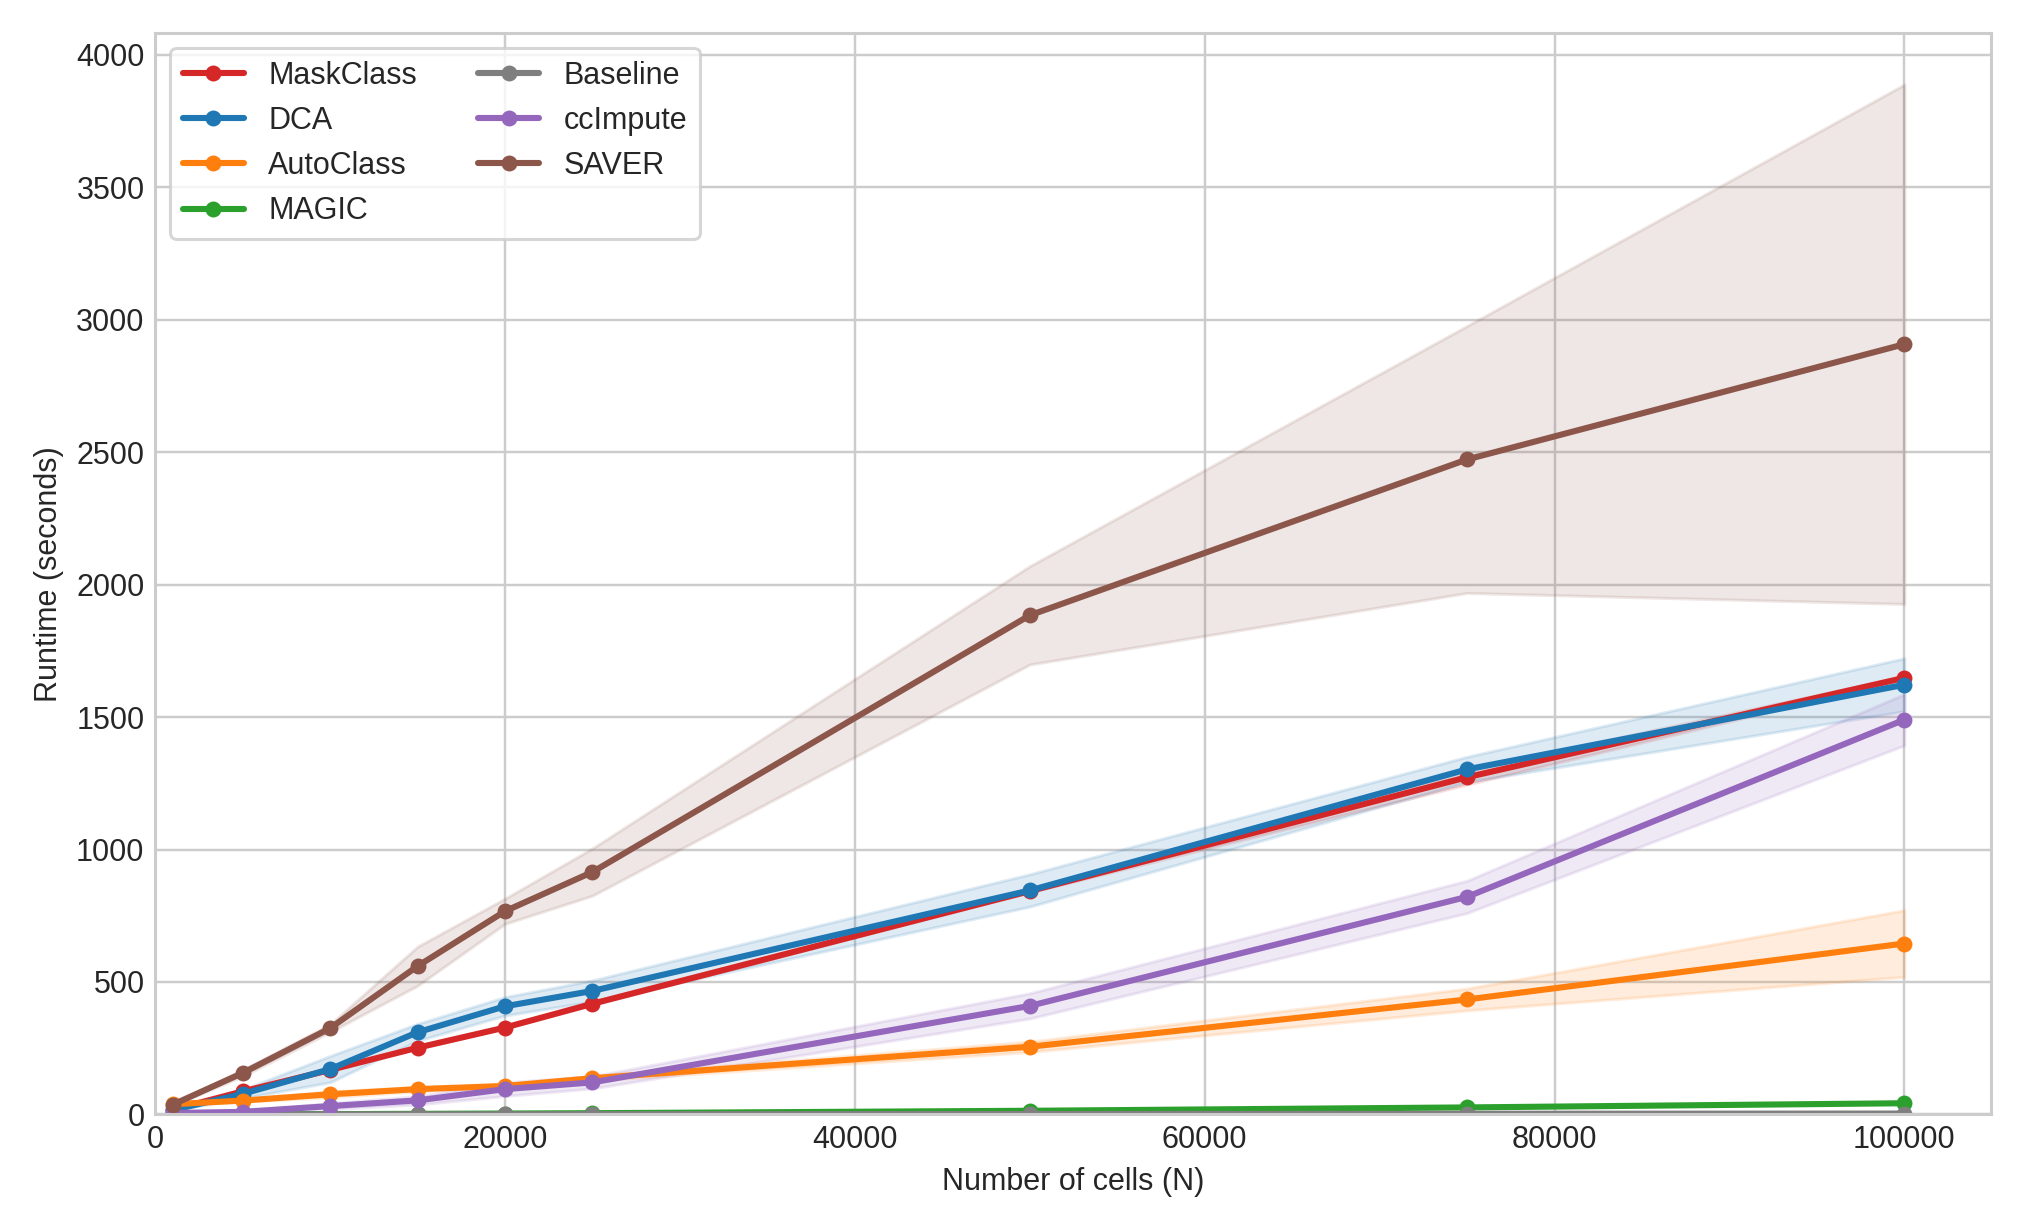
\includegraphics[width=\textwidth]{figures/runtime_scaling_linear.png}
\caption{Runtime scaling on synthetic data in linear time scale. Points show
mean runtime (seconds) across the four synthetic datasets for each cell count;
shaded regions indicate one standard deviation across datasets.}
\Description{Line chart of runtime in seconds versus number of cells on a linear y-axis for MaskClass, AutoClass, MAGIC, Baseline, ccImpute, and SAVER; SAVER ends at 50000 cells.}
\label{fig:runtime_linear}
\end{figure*}

\section{Software and Data Availability}
MaskClass source code is available at \maskclassrepolink.
The datasets used in this work are publicly available through
\ccimputedatasetslink and the original publications cited in
Section~\ref{sec:methods}.
If this paper is accepted, we will provide a versioned artifact package for
code, pre-processing scripts, and experiment configuration files to support
reproducibility.

% Acknowledgements should only appear in the accepted version.
% \section*{Acknowledgements}

% \textbf{Do not} include acknowledgements in the initial version of the paper
% submitted for blind review.

% If a paper is accepted, the final camera-ready version can (and usually should)
% include acknowledgements.  Such acknowledgements should be placed at the end of
% the section, in an unnumbered section that does not count towards the paper
% page limit. Typically, this will include thanks to reviewers who gave useful
% comments, to colleagues who contributed to the ideas, and to funding agencies
% and corporate sponsors that provided financial support.

\section{Limitations and Ethical Considerations}
This study focuses on denoising and imputation quality under common
single-cell RNA-seq settings, but it does not exhaustively cover all sequencing
platforms or domain-specific downstream endpoints. Model behavior can vary
across highly imbalanced cell populations, extreme sequencing depths, or
distribution shifts that differ from the training corpus. While we evaluate
multiple datasets and simulation scenarios, additional external validation in
new biological settings remains necessary.

The work uses public single-cell datasets and does not involve direct human
subject interaction in this study. Potential risks include misuse of imputed
signals as if they were direct measurements, which can propagate uncertainty or
bias into downstream biological interpretation. To mitigate this, we report
both recovery and clustering metrics, discuss trade-offs between dropout
recovery and preserving true zeros, and recommend domain-expert validation
before high-stakes decisions.

\bibliography{references}
\bibliographystyle{ACM-Reference-Format}
\end{document}
